\documentclass[11pt,a4paper]{article}
\usepackage[utf8]{inputenc}
\usepackage[english]{babel}
\usepackage{geometry}
\geometry{margin=1in}
\usepackage{graphicx}
\usepackage{hyperref}
\usepackage{minted}        % for code highlighting (requires -shell-escape)
\usepackage{titlesec}
\usepackage{fancyhdr}
\usepackage{caption}
\usepackage{enumitem}
\usepackage{listings}
\usepackage{xcolor}
%\usepackage{titling}
\lstset{
  basicstyle=\ttfamily\small,
  breaklines=true,
  backgroundcolor=\color{gray!10},
  frame=single,
}
\lstdefinelanguage{yaml}{
  keywords={true,false,null,y,n},
  keywordstyle=\color{blue},
  basicstyle=\ttfamily\small,
  sensitive=false,
  comment=[l]{\#},
  morecomment=[l]{\#},
  commentstyle=\color{gray}\ttfamily,
  morestring=[b]',
  morestring=[b]"
}

% Header and footer
\pagestyle{fancy}
\fancyhf{}
\rhead{Project Documentation}
\lhead{Rocket App}
\rfoot{\thepage}

% Section format
\titleformat{\section}{\normalfont\Large\bfseries}{\thesection}{1em}{}
\titleformat{\subsection}{\normalfont\large\bfseries}{\thesubsection}{1em}{}

% Title page
\title{
    \begin{flushright}
        
\includegraphics[width=5cm]{C:/Users/dfgra/OneDrive/Documents/GitHub/rocket-app/docs/images/Logo-HFT-Stuttgart.png}
    \end{flushright}
    \begin{center}
    {\huge \thetitle \par}
        \vspace{1.5cm}
        
\includegraphics[width=6cm]{C:/Users/dfgra/OneDrive/Documents/GitHub/rocket-app/docs/images/AppIcon.png} % Bild nochmal in der Mitte
        \vfill
        {\Large \theauthor \par}
        {\large \thedate \par}
    \end{center}
    \vspace{2cm}
    \Huge\textbf{Rocket App} \\
    \LARGE\textit{Pervasive Computing} \\
    \vspace{2cm}
    \large Date: \today \\
    \vfill
}
\newcommand{\email}[1]{\texttt{#1}}
\newcommand{\id}[1]{\texttt{#1}}
\author{
    Paul Durz, \id{1005080}, \email{22dupa1bif@hft-stuttgaet.de}
    \and
    Dominik Gräter, \id{1005093}, \email{22grdo1bif@hft-stuttgart.de}
    \and
    Manuel Holm, \id{1005094}, \email{22homa1bif@hft-stuttgart.de}
    \and
    Ron Seifried,\id{1005466}, \email{22sero1bif@hft-stuttgart.de}
}
\newcommand{\institute}[1]{\par\medskip\centering #1\par\medskip}

\begin{document}
\maketitle
\institute{
    Hochschule für Technik Stuttgart, Schellingstraße 24, 70174 Stuttgart, Deutschland
    \email{info@hft-stuttgart.de}
    \url{https://www.hft-stuttgart.de/}
}
\newpage
\tableofcontents
\newpage

\section{Einleitung}
Im Rahmen des Moduls Ubiquitous Computing von Professor Knauth sollten die
Studierenden das Erlernte in einem praktischen Projekt anwenden.
Das Projekt beschäftigt sich mit der Thematik des Ubiquitous Computings. Die
Durchdringung von Alltagsgegenständen mit Informationstechnologie und die
Vernetzung von smarten Systemen führen zu einer Umwelt, in der in allen Bereichen
Veränderungen auftreten. Wir haben uns dabei für eine Mobile App für Smartphones entschieden.

\subsection{Projektbeschreibung}
Die \textbf{Rocket App} ist eine mobile Anwendung, die es Nutzerinnen und Nutzern ermöglicht, ihre täglichen Schritte automatisch zu erfassen. Die App belohnt Aktivität durch ein Punktesystem, das sowohl auf der Anzahl der Schritte als auch auf der Teilnahme an Herausforderungen (Challenges) basiert. Zusätzlich können Läufe (Runs) aufgezeichnet, auf Karten dargestellt und im Nachhinein analysiert werden. Die Kombination aus Bewegungstracking, Gamification und sozialem Vergleich macht die Rocket App zu einem motivierenden Begleiter im Alltag.

\subsection{Ziele und Motivation}
Ziel der Rocket App ist es, Nutzerinnen und Nutzer zu einem aktiveren Lebensstil zu motivieren. Durch spielerische Elemente wie Punkte, Ranglisten und Challenges soll Bewegung im Alltag gefördert und langfristig zur Gewohnheit gemacht werden. Gerade im Kontext zunehmender Digitalisierung und Bewegungsmangel bietet die App eine niedrigschwellige Möglichkeit, körperliche Aktivität zu fördern und messbar zu machen.

Die Zielgruppe der App sind Menschen, die ihre Bewegung im Alltag tracken und sich selbst oder im Wettbewerb mit anderen motivieren möchten. Dazu gehören sowohl Gelegenheitsnutzer als auch sportlich Aktive.

\section{Entwicklung}
\subsection{Versionsveraltung}
Für die Entwicklung der \textbf{Rocket App} wurde ein zentrales Git-Repository unter GitHub verwendet. Im Zuge dessen haben wir eine eigene Organisation namens \texttt{RealTeamRocket} auf GitHub gegründet, um die Projektressourcen zentral zu verwalten und die Zusammenarbeit im Team zu erleichtern. Das Repository ist unter folgendem Link öffentlich einsehbar:
\url{https://github.com/RealTeamRocket/rocket-app}

Das Repository enthält sämtliche Quellcodes des Projekts – darunter das Flutter-Frontend der App, das Backend sowie eine begleitende Website. Durch diese zentrale Struktur wird sichergestellt, dass alle Komponenten konsistent versioniert und gepflegt werden können.

Zur effizienten Zusammenarbeit im Team wurde mit einem \textbf{Branching-Modell} gearbeitet. Dabei existieren Hauptzweige wie \texttt{main} und \texttt{dev}, während neue Features oder Bugfixes in separaten Feature-Branches entwickelt und anschließend via Pull Request integriert wurden. Dieses Vorgehen erlaubt paralleles Arbeiten, minimiert Merge-Konflikte und sorgt für eine saubere Trennung zwischen stabilen Releases und laufender Entwicklung.

Zur Sprint-Planung und Aufgabenverteilung kommt zusätzlich ein \textbf{GitHub Project Board} zum Einsatz, das als Kanban-Board konfiguriert wurde. Dort werden Tickets angelegt, priorisiert und den jeweiligen Teammitgliedern zugewiesen. Das Board dient als zentrale Planungsgrundlage für unsere zweiwöchigen Sprints und bietet eine transparente Übersicht über den Fortschritt einzelner Aufgaben und Meilensteine.

Durch die Kombination aus GitHub, strukturiertem Branch-Workflow und projektbezogener Aufgabenplanung konnte eine effektive und nachvollziehbare Versionskontrolle realisiert werden, die sowohl technische als auch organisatorische Anforderungen erfüllt.

\subsection{Entwicklungsumgebungen}

Für die Entwicklung der \textbf{Rocket App} kamen unterschiedliche Entwicklungsumgebungen zum Einsatz, abgestimmt auf die jeweiligen Anforderungen der Frontend- und Backend-Komponenten.

Die App wurde mit dem Framework \textbf{Flutter} entwickelt. Für die mobile Entwicklung wurde hauptsächlich \textbf{Android Studio} verwendet, insbesondere für das Erstellen, Debuggen und Testen auf realen Geräten sowie Emulatoren. Ergänzend kam auch der integrierte \textbf{Emulator von Visual Studio Code (VS Code)} zum Einsatz, insbesondere für schnelle Tests und kleinere Anpassungen während der Entwicklung. Dank der Flutter-Integration in beide Umgebungen konnten Entwickler flexibel je nach Präferenz arbeiten.

Für das \textbf{Backend}, das in der Programmiersprache \textbf{Go} entwickelt wurde, war die Wahl der Entwicklungsumgebung weitgehend frei. Da Go standardmäßig nur über den Go Language Server Protocol (gopls) unterstützt wird, kamen primär Editoren mit entsprechender LSP-Unterstützung zum Einsatz. Die bevorzugten Tools waren hier \textbf{Visual Studio Code} sowie der moderne Editor \textbf{Zed}, welcher sich durch seine Performance und klare Nutzeroberfläche auszeichnet. Beide Umgebungen bieten durch die LSP-Anbindung komfortable Features wie Autovervollständigung, Syntaxhervorhebung und Code-Navigation.

Durch diese vielseitige Toolauswahl konnten alle Projektbeteiligten in einer für sie optimalen Umgebung arbeiten, ohne auf zentrale Entwicklungsfeatures verzichten zu müssen. Dies förderte eine produktive Arbeitsweise und erhöhte die Effizienz im Entwicklungsalltag.

\subsection{Virtual Private Server}

Für das Hosting der Server-Komponenten der \textbf{Rocket App} wird ein \textbf{Virtual Private Server (VPS)} von \textbf{Oracle Cloud} genutzt. Auf diesem Server laufen sowohl das \textbf{Backend} als auch die dazugehörige \textbf{PostgreSQL-Datenbank}. Um die Dienste zuverlässig und portabel zu betreiben, werden beide Komponenten in separaten \textbf{Docker-Containern} ausgeführt.

Die Orchestrierung dieser Container erfolgt über eine \textbf{Docker Compose}-Konfiguration, die das Starten, Stoppen und Verwalten der Services vereinfacht. Zusätzlich kommt das Tool \textbf{Watchtower} zum Einsatz, das regelmäßig nach aktualisierten Docker-Images prüft. Sobald ein neues Image – beispielsweise des Backends – auf \textbf{Docker Hub} verfügbar ist, lädt Watchtower es automatisch herunter und startet den entsprechenden Container neu. Dadurch wird sichergestellt, dass der Server stets mit der aktuellsten Version läuft, ohne manuelles Eingreifen.

\subsection{Deployment}

Das Deployment des Backends ist vollständig automatisiert und in den Entwicklungsworkflow über \textbf{GitHub-Actions} integriert. Bei jedem \textbf{Pull Request auf den \texttt{master}-Branch}, der Änderungen im Verzeichnis \texttt{rocket-backend} betrifft, wird eine entsprechende GitHub-Action ausgelöst.

Diese Action übernimmt das Erstellen eines neuen Docker-Images auf Basis des aktuellen Codes und lädt es anschließend in ein zentrales \textbf{Docker Hub}-Repository hoch. Sobald das neue Image dort verfügbar ist, erkennt \textbf{Watchtower} auf dem Oracle-Server das Update und sorgt automatisch für einen nahtlosen Rollout der neuen Backend-Version.

Ein Ausschnitt aus dem verwendeten Deployment-Workflow sieht wie folgt aus:

\begin{lstlisting}[language=yaml, caption={GitHub Action zur automatisierten Bereitstellung}, label={lst:deployment}]
name: Build and Push Docker Image

on:
  push:
    branches:
      - master
    paths:
      - 'rocket-backend/**'

jobs:
  build-and-push:
    runs-on: ubuntu-latest

    steps:
      - name: Checkout code
        uses: actions/checkout@v3

      - name: Log in to Docker Hub
        uses: docker/login-action@v2
        with:
          username: ${{ secrets.DOCKER_USERNAME }}
          password: ${{ secrets.DOCKER_PAT }}

      - name: Set up Docker Buildx
        uses: docker/setup-buildx-action@v2

      - name: Build and Push Docker Image
        uses: docker/build-push-action@v4
        with:
          context: ./rocket-backend
          push: true
          tags: ${{ secrets.DOCKER_USERNAME }}/rocket-backend:latest
\end{lstlisting}

Durch diese Pipeline wird das Deployment effizient, reproduzierbar und sicher gestaltet – ein entscheidender Vorteil bei der iterativen Weiterentwicklung der Rocket App.


\section{Systemarchitektur}
\begin{enumerate}
    \item Prerequisites (e.g., Node.js, Python)
    \item Installation steps
\end{enumerate}
\subsection{Backend}
\subsubsection{Umsetzung}
\subsection{Frontend}
\subsubsection{Umsetzung}
\subsection{Schwierigkeiten}
Schwierigkeiten waren vor allem das Anzeigen eines "getrackten Runs" auf der OSM-Karte. Ein Run besteht aus mehreren GPS-Punkten, diese sollen auf der Karte angezeigt werden.
Das Problem war, dass die map_controller.dart den RoadType.foot nur für Routen zwischen zwei Punkte anzeigt. Also haben wir die Route in mehrere kleine Routen unterteilt, sodass die Karte diese anzeigt.\\
\section{Extra/Website}
Für die Möglichkeit, die App mit einer Website erweitern zu dürfen, danken wir Professor Dr. Knauth und Prof. Dr. Mosler.
Diese Erweiterungen und Darstellung der App auf einer Website sind nicht Teil der Pervasive Computing Vorlesung, gehören aber zu unserem Projekt dazu und sollten hier nicht unerwähnt bleiben.
Die Website bietet die selben Features wie die App, man kann aber auch noch Runs planen, man hat einen globalen Chat und man hat die Möglichkeit die App zu downloaden.
Hier ist noch das ER-Modell der Website:
\begin{figure}[h]
    \centering
    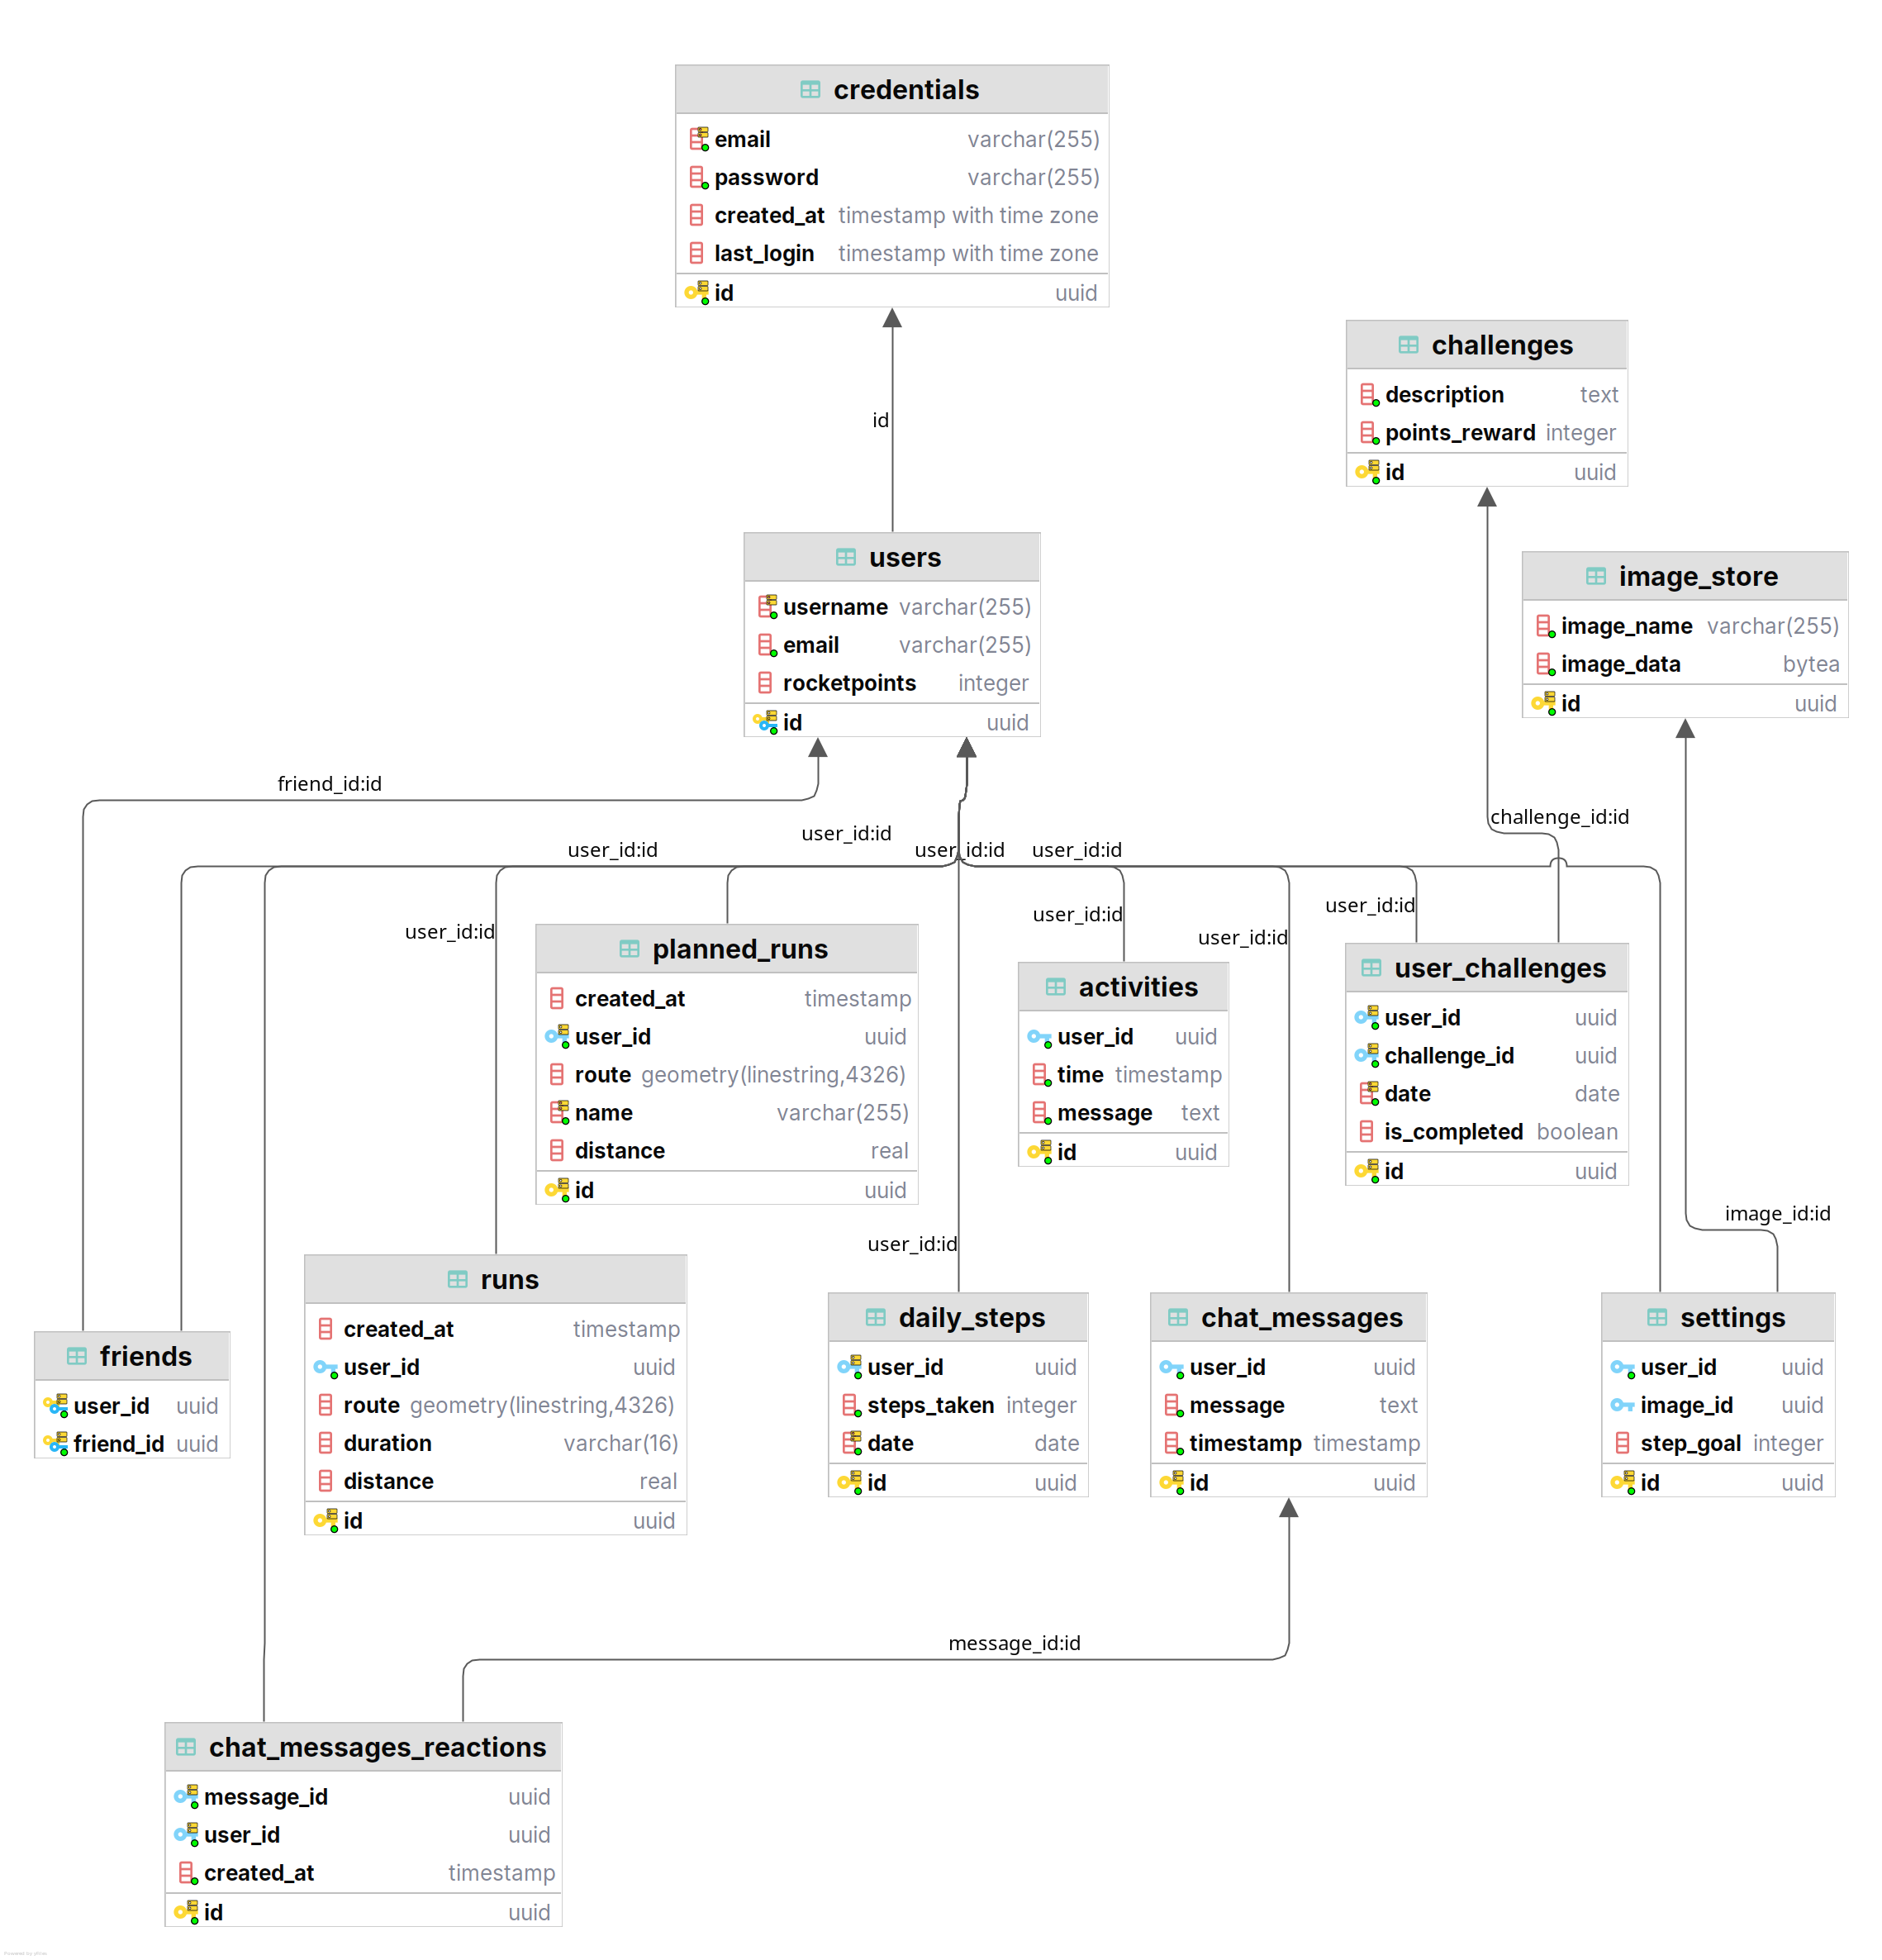
\includegraphics[width=0.8\textwidth]{C:/Users/dfgra/OneDrive/Documents/GitHub/rocket-app/docs/images/RocketERLight.png}
    \caption{ER-Modell der Website}
    \label{fig:er-model-website}
\end{figure}
\section{Fazit}
\section{Zeiterfassung}
Wir haben unsere Zeiten mit dem Tool \textbf{Clockify} erfasst. Dieses Tool ist zwar etwas schwächer als Everhour. Aber es ist kostenlos und man konnte seine Zeiten schnell und einfach erfassen.\\
Hier eine Übersicht der erfassten Zeiten:
\begin{figure}[h]
    \centering
    
\includegraphics[width=0.8\textwidth]{C:/Users/dfgra/OneDrive/Documents/GitHub/rocket-app/docs/images/AppIcon.png}
    \caption{Clockify Zeiterfassung}
    \label{fig:clockify}
\end{figure}
\section{Quellen}
\begin{thebibliography}{8}
    \bibitem{ref_url1}
    OSM Wiki, \url{https://wiki.openstreetmap.org/wiki/DE:Hauptseite}, letzter Zugriff am 14.5.2025.
    \bibitem{ref_url2}
    Flutter Homepage, \url{https://flutter.dev/}, letzter Zugriff am 4.4.2025.
    \bibitem{ref_url3}
    Android Studio, \url{https://developer.android.com/studio}, letzter Zugriff am 4.4.2025.
    \bibitem{ref_url4}
    Clockify, \url{https://clockify.me/}, letzter Zugriff am 24.6.2025.
\end{thebibliography}
\end{document}

